\documentclass[11pt,a4paper]{report}
\usepackage[utf8]{inputenc}
\usepackage[french]{babel}
\usepackage[T1]{fontenc}
\usepackage{amsmath}
\usepackage{amsfonts}
\usepackage{amssymb}
\usepackage{xcolor}
\usepackage{gensymb}

\usepackage{geometry}
\geometry{hmargin=2.5cm,vmargin=1.5cm}
\usepackage{wasysym}
\usepackage{graphicx}

\author{Mathieu Sarrat}
\title{LC1 - Chimie et Couleur}

\makeatletter
\renewcommand{\thesection}{\@arabic\c@section}
\makeatother


\begin{document}
\maketitle

\section*{Niveau, Pré-requis et objectifs}
\begin{itemize}
	\item \textbf{Niveau :} Première S\\
	
	\item \textbf{Pré-requis :}
	\begin{itemize}
		\item Synthèse additive et soustractive de la couleur;
		\item Formules brute, développée, semi-développée;
		\item Réaction d'oxydoréduction;
		\item Tableau d'avancement, rendement d'une réaction.\\
	\end{itemize}
	
	\item \textbf{Objectifs :}
	\begin{itemize}
		\item Introduire la représentation topologique;
		\item Établir un lien entre la couleur et la structure des molécules;
		\item Introduire la loi de Beer-Lambert;
		\item Synthétiser un colorant;
		\item Dosage spectrophotométrique par étalonnage.\\
	\end{itemize}
		
	\item \textbf{Recommandations :}
	\begin{itemize}
		\item Synthétiser l'indigo en premier. Une première fois en totalité (jusqu'à l'étude). Refaire 		et s'arrêter avant la filtration.
		\item Courbe d'étalonnage pour le dosage du bleu patenté : faire 5 points.\\
	\end{itemize}
	
	\item \textbf{Bibliographie :}
	\begin{itemize}
		\item Terminale S Hachette. Physique Chimie Enseignement Spécifique, pour le dosage.
		\item Première S pour le cours.
		\item Le Maréchal Tome 2
		\item Chimie des couleurs et des odeurs (synthèse de l'indigo).
	\end{itemize}
\end{itemize}

\newpage
\section*{Introduction}

La couleur peut être définie comme la qualité de la lumière renvoyée par la surface d'un objet. Elle correspond aussi à la sensation perçue par le cerveau quand l’œil lui transmet le signal d'une lumière correspondant à un intervalle donné de fréquence.\\

Les matières colorées sont utilisées depuis la Préhistoire. Des fresques peintes (cf. peintures rupestres de la grotte de Lascaux) avec des matières colorées minérales, telles que l'ocre, la craie ou le noir de charbon, ont été retrouvées dans des grottes ornées de peintures rupestres. Dès l'Antiquité on sait extraire des matières colorées des végétaux, comme la garance ou l'indigo; ou d'animaux, comme la cochenille des teintures et le murex, coquillage duquel les Romains tiraient la pourpre.

\begin{figure}[h!]
	\begin{center}
		\begin{tabular}{cc}
  		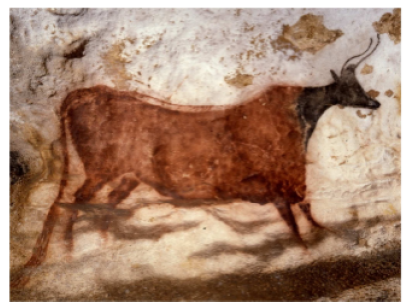
\includegraphics[scale = 0.7]{lascaux1.png} &
   		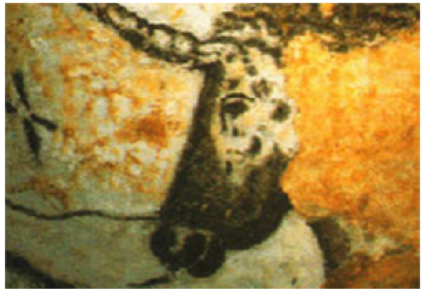
\includegraphics[scale = 0.7]{lascaux2.png}\\
	\end{tabular}
	\caption{Peintures rupestres de la grotte de Lascaux.}
	\end{center}
\end{figure}

Leur extraction était souvent longue et laborieuse, leur fixation sur support parfois imparfaite et leur coût de revient élevé. Dès le milieu du $\text{XIX}^e$ siècle, les chimistes parviennent à synthétiser des espèces chimiques colorées, c'est par exemple le cas de la mauvéine synthétisée par Perkin en 1856. Cette avancée s'inscrit dans le contexte de grands progrès en chimie organique, la chimie des molécules contenant en majorité les atomes C et H, très présentes dans la matière vivante.\\

Les matières colorées naturelles sont alors progressivement remplacées par des produits de synthèse. De nos jours, une matière colorée peut être organique ou inorganique, naturelle ou synthétique. 

\newpage
\section{Origines chimiques de la couleur}\label{sec:1}

\subsection{Pigments et colorants}

Les molécules colorées sont classées en deux catégories suivant leur solubilité dans le solvant, les \textbf{colorants} et les \textbf{pigments}.\\ 

\begin{itemize}
	\item Les colorants sont des espèces solubles dans le milieu qu'ils colorent. On les trouve dans 		l'alimentation, en particulier dans les boissons et dans les bonbons. On en trouve aussi dans les 		encres pour teindre les vêtements.\\
	
	\item Toute comme un colorant, les pigments colorent un milieu, mais ils se présentent sous forme 		d'une poudre insoluble. Il est donc important de choisir un milieu qui puisse maintenir les 			pigments sans qu'il n'y ait décantation. Un tel milieu est appelé un \textbf{liant}. Il s'agît par 		exemple des huiles utilisées en peinture. Dans ce cas, le liant remplit trois fonctions : donner de 	la cohésion aux pigments pour pouvoir manipuler la peinture (on forme une pâte plus ou moins 			fluide), permettre à la matière colorée de sécher et durcir pour former un film solide et durable, 		réversible (gouache) ou non (acrylique) et enfin donner un aspect particulier à la peinture (mat, 		brillant, etc...).	
\end{itemize}

\subsection{Synthèse de l'indigo (Le Maréchal, Tome 2, p137 et 138.)}
Les pigments et les colorants peuvent être extraits de substances naturelles ou synthétisés. Par exemple, l'indigo peut être extrait d'une plante, l'indigotier, ou synthétisé à partir de produits
chimiques, ce qui permet de réduire sont prix de revient. 

\subsubsection{Synthèse de l'indigo}
 La réaction de synthèse est la suivante :
\begin{equation}
	2{\text{C}_7\text{H}_5\text{NO}_3}_\text{(s)} + 2{\text{C}_3\text{H}_6\text{O}}_\text{(l)} 
	+ 2{\text{HO}^{–}}_\text{(aq)}  = {\text{C}_{16}\text{H}_{10}\text{N}_2\text{O}_2}_\text{(s)}
	+ 2{\text{CH}_3\text{CO}_2}^{–}_\text{(aq)} + 4{\text{H}_2\text{O}}_\text{(l)}	 
\end{equation}

\textit{Ils n'ont pas encore vu la représentation topologique, on donne les formules brutes, en indiquant sous chaque expression le nom de la molécule. On donnera les représentations topologiques plus loin, après avoir défini cette représentation.}\\

\begin{itemize}
	\item \textbf{En préparation :}
	\begin{itemize}
		\item Dans un tube à essais, dissoudre 0.5g de 2-nitrobenzaldéhyde (3.3 mmol) dans 5 mL 					d'acétone, qui sert de réactif et de solvant.
		\item Saisir le tube à essais avec une pince en bois (la réaction est exothermique) et 						introduire goutte à goutte 2.5 mL de soude à 1 mol. Cela chauffe et peut bouillir.
		\item Laisser réagir 5 minutes.
		\item Filtrer sur fritté et laver avec 10 mL d'eau distillée, puis 10 mL d'éthanol à 95\%. Le 				lavage à l'éthanol permet d'éliminer les restes de 2-nitrobenzaldéhyde.
		\item \textbf{Peser la coupelle qui va recueillir l'indigo.}
		\item Sécher le solide à l'étuve (100-120 \degree C) pendant 40 min.
		\item Relancer une seconde synthèse, s'arrêter avant la filtration.\\
	\end{itemize}
	
	\item \textbf{En direct :}
	\begin{itemize}
		\item Présenter la réaction.
		\item Faire la filtration de la seconde synthèse et présenter le dispositif Buchner.
		\item Dresser un tableau d'avancement, montrer qui est le réactif limitant (2-nitro...), 					calculer l'avancement maximal et la masse maximale d'indigo que l'on peut produire :
		\begin{equation}
			m(In)_\text{max} = \xi_\text{max} M(In),
		\end{equation}
		avec M(In) $=$ 262.3 g/mol et M(2-nitro) $=$ 151.12 g/mol.
		
		\item Calculer le rendement 
		\begin{equation}
			\eta = \frac{m(In)_\text{pesée}}{m(In)_\text{max}}
		\end{equation}
		à partir de l'échantillon placé à l'étuve.
	\end{itemize}
\end{itemize}

\subsubsection{Utilisation en teinture}

Pour colorer un tissu, comme un jean, il faudrait mettre l'indigo en solution pour imbiber les fibres. Or, l'indigo est insoluble dans l'eau. On doit donc le transformer en composé soluble.

\begin{itemize}
	\item Erlenmeyer : dissoudre 0.5g de dithionite de sodium dans 40 mL d'eau distillée avec une 				pastille de soude et un peu de pierre ponce.
	\item Faire chauffer jusqu'à ébullition.
	\item Ajouter 0.1g d'indigo et \textbf{boucher l'erlenmeyer}, pour éviter l'oxydation par le 				dioxygène de l'air.
	\item Agiter la solution jusqu'à ce que l'indigo soit dissout. La solution prend une 						teinte verte. Ajouter plus de dithionite de sodium si l'indigo n'est pas entièrement dissous.
	\item Immerger un échantillon de tissu/de coton dans la solution à l'aide d'une baguette de verre. 			Reboucher. Agiter 30 secondes. 
	\item Retirer l'échantillon, laisser à l'air libre pour le sécher : le dioxygène de l'air oxyde la 			forme leuco, et la teinte bleue apparaît. Laver pour retirer l'indigo qui ne s'est pas fixé, 			ainsi que les restes éventuels de dithionite de sodium et de soude. On ne lave qu'après la 				réoxydation de l'indigo, une fois qu'il est devenu insoluble.\\
	\end{itemize}

La réaction entre l'indigo et les ions dithionate est une réaction d'oxydoréduction au cours de laquelle l'indigo est réduit par les ions dithionite en forme "leuco" et les ions dithionite 
${\text{S}_2\text{O}_4}^{2-}$ sont oxydés en ions sulfite ${\text{SO}_3}^{2-}$ :
	\begin{equation}
		\text{In} + 4\text{HO}^- + {\text{S}_2\text{O}_4}^{2-} 
		= \text{In}^{2-} + 2\text{H}_2\text{O} + 2{\text{SO}_3}^{2-}.
	\end{equation}
\textit{On écrit la demi-équation d'oxydation des ions dithionite en milieu basique.}
On forme la forme leuco (en réalité jaune) de l'indigo, soluble dans l'eau et permettant une teinte en profondeur de la fibre du tissu. Le dioxygène oxyde ensuite la forme leuco en indigo, selon la réaction
\begin{equation}
	\text{In}^{2-} + \frac{1}{2}\text{O}_2 + \text{H}_2\text{O} = \text{In} + 2\text{HO}^{-}.
\end{equation}
\textit{On écrit la demi-équation de réduction du dioxygène en milieu basique.}
\subsection{Couleur et structure moléculaire}

En interagissant avec la lumière, les molécules absorbent une partie de l'énergie lumineuse correspondant à certaines fréquences. La lumière qui n'a pas été absorbée est diffusée, collectée par l'œil et nous la percevons sous forme de couleur. On peut alors se doute que l'organisation de la matière, et notamment la structure des molécules, va avoir un rôle à jouer dans la couleur d'une substance.

\subsubsection{Molécules organiques}

Historiquement une molécule organique est une molécule provenant d'un organisme vivant. Au $\text{XIX}^e$ siècle, les chimistes ont commencé à synthétiser des molécules similaires aux molécules naturelles.
Aujourd'hui, on définit les molécules organiques comme molécules constituées essentiellement de l'élément carbone C et l'élément hydrogène H.\\

Une molécule organique est formée d'un \textbf{enchaînement plus ou moins long d'atomes de carbone
qui constituent le squelette} de la molécule. Ceux-ci sont principalement liés à des atomes
d'hydrogène, mais on trouve aussi des groupes contenant d'autres éléments chimiques (oxygène, soufre, azote, chlore, etc...) : ce sont des \textbf{groupes caractéristiques}, qui confèrent à une molécule un certain nombre de propriétés.

\subsubsection{Représentation topologique d'une molécule}

Jusqu'ici nous avons représenté les molécules par leur formule brute, par exemple celle de l'indigo
\begin{equation}
	\text{C}_{16}\text{H}_{10}\text{N}_2\text{O}_2.
\end{equation}
Cette formule ne nous apporte aucune information sur l'arrangement des atomes les uns par rapport aux autres, d'où le recours aux formules développées ou semi-développées pour se faire une idée de cet arrangement.\\

Les molécules organiques possèdent souvent un grand nombre d'atomes, et ces représentations peuvent devenir fastidieuses, d'où le recours à une représentation simplifiée, \textbf{la représentation topologique} :
\begin{itemize}
	\item les liaisons carbone-carbone sont représentées par des segments;
	\item les doubles liaisons sont représentées par des doubles segments;
	\item les hétéro-atomes (ceux qui ne sont ni C, ni H) sont tous représentés;
	\item les atomes d'hydrogène portés par les hétéroatomes sont représentés;
	\item les atomes d'hydrogène \textbf{portés par les atomes de carbone ne sont pas représentés}.
		Les atomes de carbone en portent autant que nécessaire pour établir au total 4 liaisons 				covalentes (4 simples, ou 2 simples et une double par exemple).
\end{itemize}

Quelques exemples : \textcolor{red}{faire le cas du propane puis de l'éthanol à la main, puis montrer une diapo avec d'autres exemples et notamment les espèces impliquées dans la synthèse de l'indigo.}

\subsubsection{Chromophores et auxochromes}

Les liaisons entre atomes sont assurées par des doublets d'électrons. L'interaction de la lumière
avec la matière dépend de l'énergie des électrons des molécules et \textbf{plus particulièrement de ceux des doubles liaisons} :
\begin{itemize}
	\item les molécules colorées présentent une \textbf{alternance régulière de doubles liaisons et de 			simples liaisons} : on dit que les doubles liaisons sont conjuguées;
	\item les molécules colorées absorbent certaines longueurs d'onde du domaine visible. La couleur
		perçue correspond à la couleur complémentaire des radiations absorbées;
	\item \textbf{la longueur d'onde de la lumière observée augmente lorsque le nombre de doubles 				liaisons conjuguées augmente}. En dessous de 7 doubles liaisons conjuguées, l'absorption se 			fait dans le domaine des ultraviolets ce qui ne donne pas de coloration perceptible pour les 			humains.
\end{itemize}

La transformation de la lumière blanche en lumière colorée résulte de l'absorption sélective d'énergie par certains groupes d'atomes appelés \textbf{chromophores} :
\begin{equation}
	-C = C - C = C - \quad;\quad - C = N - \quad;\quad  -N = N- \quad;\quad  -C = C - C = O.
\end{equation}
\textit{Hors programme : Ils disposent d'orbitales vides ou incomplètes à des niveaux d'énergie peu éloignés de ceux des orbitales remplies, de sorte qu'ils absorbent la lumière visible d'énergie correspondant aux transitions possibles entre ces niveaux.}\\ 

Dans le cas de la molécule d'indigo, c'est la délocalisation des doublets électroniques des atomes d'azote qui permet de "mettre en contact" les chaînes d'alternance de double/simple liaisons et donc de faire de l'indigo une molécule colorée.\\

\begin{figure}[h!]
	\begin{center}
		\begin{tabular}{cc}
  		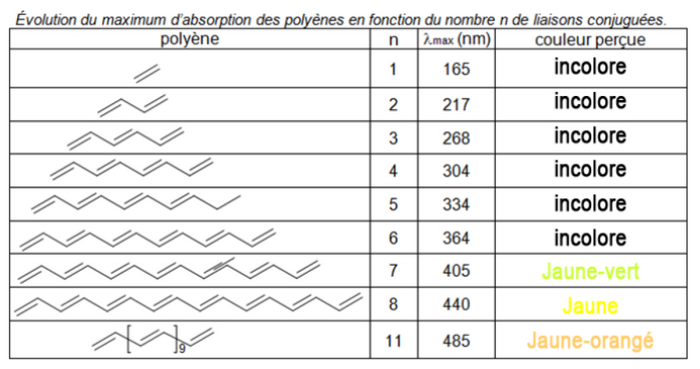
\includegraphics[scale = 0.5]{alternance.png} &
   		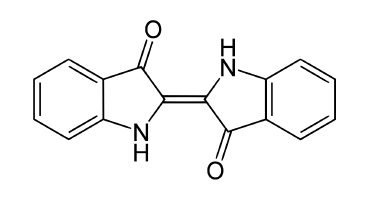
\includegraphics[scale = 0.7]{indigo.png}\\
	\end{tabular}
	\caption{Gauche : polyènes. Droite : indigo.}
	\end{center}
\end{figure}

La \textbf{présence de substituants} peut modifier la longueur d'onde d'absorption : ils jouent le rôle de \textbf{groupes auxochromes} en déplaçant le maximum d'absorption vers de plus grandes longueurs d'onde. Ainsi, une molécule qui, sans groupement absorberait dans l'ultraviolet, va pouvoir absorber dans le visible et donc être colorée. Parmi ces
substituants, on peut citer :
\begin{equation}
		- \text{NH}_2 \quad;\quad -\text{OH} \quad;\quad -\text{O}-\text{CH}_3
\end{equation}

\textcolor{red}{Montrer le parallèle entre anthraquinone et alizarine.}
\begin{figure}[h!]
	\begin{center}
		\begin{tabular}{cc}
  		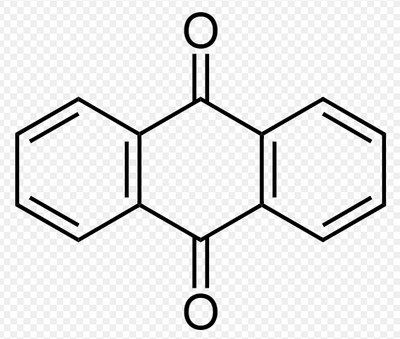
\includegraphics[scale = 0.4]{anthraquinone.png} &
   		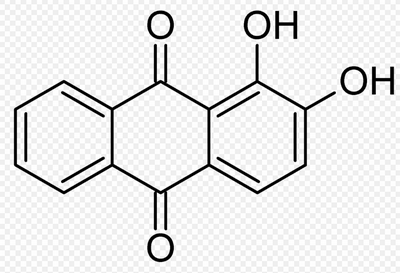
\includegraphics[scale = 0.45]{alizarine.png}\\
   		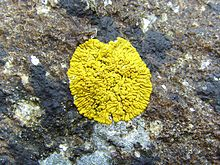
\includegraphics[scale = 0.7]{anthraquinone_ex.png} &
   		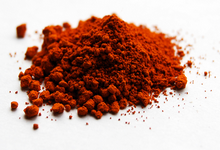
\includegraphics[scale = 0.7]{alizarine_ex.png}\\
	\end{tabular}
	\caption{Gauche : anthraquinone. Droite : alizarine.}
	\end{center}
\end{figure}


\newpage
\section{Influence de paramètres extérieurs à la molécule}\label{sec:2}

\subsection{Influence du pH}

\subsubsection*{Indicateurs colorés}

En changeant la valeur du pH de la solution dans laquelle se trouve une molécule organique, on peut
modifier cette molécule, et il peut donc y avoir changement de la couleur de la solution. C'est le cas
des espèces acido-basiques dont l'acide et la base ont des couleurs distinctes. Dans ce cas, suivant
la valeur du pH, la forme acide ou basique est majoritaire et impose sa couleur. C'est par exemple le cas avec la \textbf{phénolphtaléine} :

\textcolor{red}{Manip : deux béchers d'eau distillée, contenant de la phénolphtaléine. On verse dans l'un de l'acide chlorhydrique (1 mol/L), dans l'autre de la soude (1 mol/L). On mesure le pH. Ne pas dépasser 12, sans quoi la phénolphtaléine redevient incolore.}

\begin{figure}[h!]
	\begin{center}
		\begin{tabular}{cc}
  		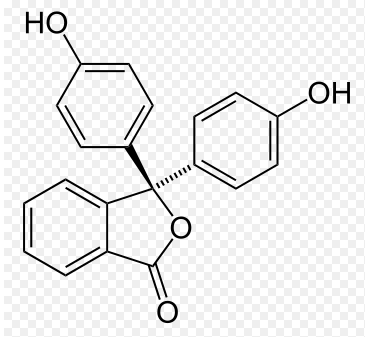
\includegraphics[scale = 0.4]{fifiacide.png} &
   		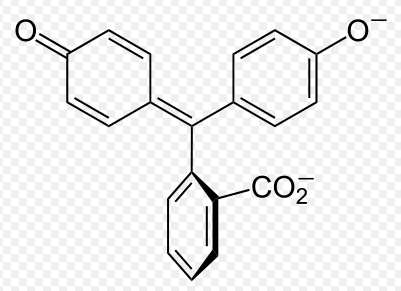
\includegraphics[scale = 0.4]{fifibasique.png}\\
	\end{tabular}
	\caption{Formes acide et basique de la phénolphtaléine.}
	\end{center}
\end{figure}

La forme acide de la phénolphtaléine présente un nombre insuffisant de doubles liaisons carbone carbone alternées simple/double. Ce n'est pas le cas de la forme basique. Il existe un grand nombre d'indicateurs colorés, dont les zones de virage (la plage de valeurs de pH dans laquelle l'indicateur change de couleur) diffèrent sensiblement \textcolor{red}{(voir diapo)}.

\subsubsection*{Les anthocyanes du jus de chou rouge}

Le chou rouge contient des anthocyanes qui, suivant le pH, adoptent l'une de leurs quatre formes (cation avylium (rouge), base quinionique (bleu-mauve), base carbinol (incolore) et chalcone (jaune clair)). La forme majoritaire impose sa couleur ; la large gamme de couleur est due à la grande variété d'espèces colorées du chou rouge. \textcolor{red}{S'il reste du temps, on peut faire l'expérience en préparation, et présenter les tubes à essais lors de la leçon (voir en Annexe pour le protocole).}

\begin{figure}[h!]
	\begin{center}
  		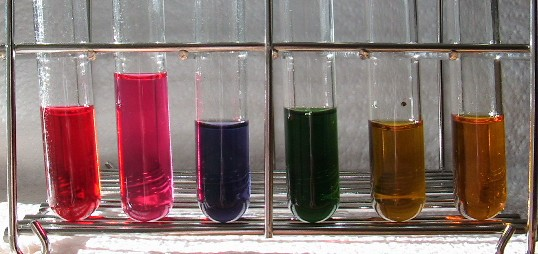
\includegraphics[scale = 0.4]{chourouge.png}
	\caption{Jus de chou rouge dilué avec ajout de produits acides ou basiques : tube 5 (rouge), tube 3 	(rose), tube 1 (bleu), tube 7 (vert), tube 8 (jaune-vert), tube 9 (jaune). Tube 5 : ajouter une 		dizaine de goutte d'acide chlorhydrique. Constater que la couleur reste rouge et n'évolue plus 			quand on ajoute encore de l'acide. Tube 3 : ajouter une ou deux gouttes d'acide éthanoïque, ou de 		vinaigre d'alcool. La couleur vire au rose fuchsia. Tube 1 : ne rien y ajouter ! Il s'agit du tube 		de la couleur de référence, "neutre", du chou rouge. La couleur est normalement bleue. Tube 7 : 		ajouter une goutte d'ammoniaque. La couleur devient d'un vert vif. Tube 8 : ajouter une goutte 			d'une solution d'hydroxyde de sodium. La couleur devient jaune-vert. Tube 9 : ajouter plusieurs 		gouttes d'une solution d'hydroxyde de sodium. Constater que la couleur devient jaune vif et 			n'évolue plus quand on ajoute encore de la soude.}
	\end{center}
\end{figure}

\subsection{Influence du solvant}

Certaines espèces chimiques ont des couleurs différentes selon le solvant dans lequel elles sont dissoutes.

\begin{itemize}
	\item Matériel : 2 tubes à essai avec bouchons, spatule, cristaux de diiode;	
	\item Introduire à la spatule un peu de diiode dans chaque tube à essai. Vers 2mL d'eau distillée 			dans un tube, 2mL de cyclohexane dans l'autre. Boucher, agiter, observer;
	\item  \textit{Explication, hors programme : le diiode adopte une coloration différente dans l'eau 			et le cyclohexane. Le diiode est un composé apolaire qui se dissout mal dans l'eau, dans 				laquelle il se présente préférentiellement sous la forme triiodure ($\text{I}_3^-$), un 				complexe de couleur jaune pâle. La molécule de diiode se dissout mieux dans le cyclohexane, 			auquel elle confère une couleur violette.}
\end{itemize}


\subsection{Influence de la température}

La température peut aussi avoir effet sur la couleur de certaines substances : on parle de \textbf{thermochromisme}. La lumière elle-même peut modifier la couleur d'un matériau, c'est par exemple le cas des verres de lunettes \textbf{photochromes} qui se teintent lorsque la quantité d'ultraviolet atteignant le verre dépasse un seuil.

\newpage
\section{Influence de la concentration}

Une solution se comporte comme un filtre coloré, lorsqu'elle est traversée par une lumière blanche. En effet, elle absorbe une partie du rayonnement et toutes les radiations ne sont pas absorbées de la même manière, d'où la couleur et ses nuances.

\subsection{Absorbance et spectrophotométrie}

L'absorbance est une grandeur physique qui traduit la capacité d'un milieu a absorber un rayonnement. Supposons qu'une seule espèce absorbe dans la solution. On peut calculer cette grandeur grâce à la loi de Beer-Lambert modélise une relation de proportionnalité entre l'absorbance et la concentration en espèce absorbante :
\begin{equation}
	\boxed{A = k C},
\end{equation}
où $C$ est la concentration en espèce absorbante, donnée en mol/L et $k$ une constante de proportionnalité dépendant de la longueur d'onde, du solvant et de l'épaisseur de solution traversée. L'absorbance est une \textbf{grandeur sans unité}. Comme toute loi, elle a un domaine de validité : il ne doit pas y avoir de solides dans la solution et les solutions doivent être diluées (concentration inférieure à $10^{-2}$ mol/L.\\

L'absorbance est donc \textbf{définie pour une longueur d'onde donnée} et on peut la mesurer grâce à un spectrophotomètre. Le principe est le suivant : une source lumineuse de longueur d'onde ajustable éclaire une cuve contenant la solution colorée à étudier. Un photo-détecteur mesure l'intensité transmise par la solution. Afin de s'affranchir de l'absorption possible par le solvant et par la cuve, un étalonnage avec du solvant pur est nécessaire : on \textbf{fait le blanc}.\\

Pour une longueur d'onde donnée, une valeur A $=$ 0 signifie que la solution est complètement
transparente : la radiation incidente n'est pas du tout absorbée. Une valeur A $=$ 1 signifie que 90
\% de l'énergie lumineuse de la radiation incidente est absorbée.\\

Le spectre d'absorption d'une solution est le graphique représentant son absorbance $A$ en fonction
de la longueur d'onde.

\textcolor{red}{Manip : spectre d'absorption du bleu patenté V :}
\begin{itemize}
	\item Faire le blanc.
	\item Tracer le spectre d'absorption du sirop de menthe.
	\item Comparer à celui du bleu patenté V (colorant E131). Il se pourrait qu'une second pic 					apparaisse, dans le violet, lié à la tartrazine du sirop de menthe. Cette espèce n'absorbe pas 			à la même longueur d'onde, donc aucun impact sur le dosage à $\lambda_\text{max}$ du bleu 				patenté. On pourrait faire une CCM pour montrer les deux espèces...
	\item Pic d'absorption maximal (dans le rouge, $\lambda = 640$ nm).
\end{itemize}

\begin{figure}[h!]
	\begin{center}
	\begin{tabular}{cc}
	  	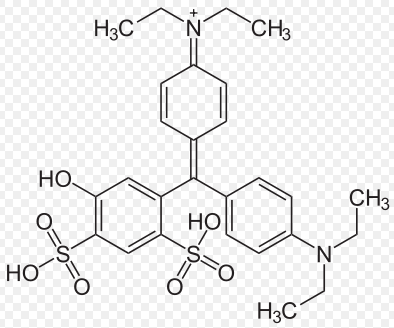
\includegraphics[scale = 0.6]{bleup.png} &
   		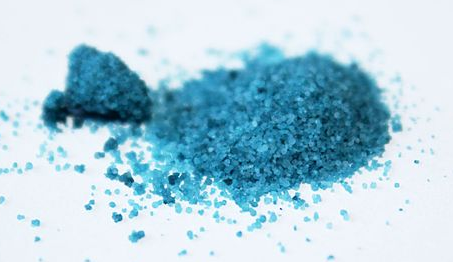
\includegraphics[scale = 0.6]{bleupex.png}\\
	\end{tabular}
	\caption{Bleu patenté V.}
	\end{center}
\end{figure}

\subsection{Dosage par étalonnage : colorant E131 dans le sirop de menthe}

La toxicité du bleu patenté, colorant alimentaire E131, est mal connue. On le soupçonnerait notamment d'aggraver ou de provoquer l'hyperactivité chez certains enfants. Interdit dans certains pays, il est cependant autorisé en Europe, où il est utilisé en médecine (en cancérologie, notamment) ou dans la confiserie. On le trouve également dans certains sirops de menthe \footnote{\textcolor{red}{Si pas de sirop de menthe, il reste le bonbon Schtroumpf, ou, à défaut, préparer une solution de bleu patenté de concentration connue.}}.\\  

La dose journalière admissible (DJA) est la dose d'additif qu'une personne peut ingérer tous les jours de sa vie sans risque appréciable pour sa santé, c'est à dire sans effet secondaire. Elle est en moyenne 100 fois inférieure à la dose pour laquelle on a vu, dans les études toxicologiques, apparaître un risque. Dans le cas du bleu patenté elle est de $2.5 \text{mg}/\text{kg}$ de masse corporelle. \textbf{Un enfant boit 0.2 L de sirop de menthe : on veut déterminer la quantité de bleu patenté qu'il ingère et la comparer à la DJA. Pour cela, on va réaliser un dosage spectrophotométrique par étalonnage.}\\

Un dosage par étalonnage consiste à \textbf{déterminer la concentration d'une espèce en solution en comparant une grandeur physique}, caractéristique de la solution, \textbf{à la même grandeur physique mesurée pour des solutions étalon}. Dans le cas du dosage du bleu patenté, cette grandeur physique est l'absorbance de la solution. Pour le dosage, nous avons \textbf{besoin de réaliser une gamme de solutions étalon}, c'est à dire de concentrations parfaitement connues.

\subsubsection*{En préparation :}
\begin{itemize}
	\item Fabriquer la gamme de solutions étalon (se reporter au livre).
	\item Tracer la droite d'étalonnage.
	\item Préparer la solution de sirop de menthe, diluer si besoin.
\end{itemize}

\subsubsection*{En direct :}
\begin{itemize}
	\item Présenter la droite d'étalonnage et la gamme étalon (sous forme d'un tableau),
	\item Expliquer la modélisation linéaire (si $C = 0$, l'absorbance doit être nulle).\\
\end{itemize}  

\textcolor{blue}{Manip :} mesurer l'absorbance du sirop de menthe, relever la concentration, calculer la masse de bleu patenté dans 0.2 L de bleu patenté. Conclure sur la DJA.
Masse molaire $\text{M(E131)} = 1159,4 \text{g}.\text{mol}^-1$.\\

\newpage
\section*{Conclusion}

La couleur est la perception que nous avons d'un rayonnement lumineux. Nous avons vu que nous pouvions relier la couleur d'une substance à ses propriétés microscopiques, c'est à dire à la structure des molécules. La couleur d'une espèce est due aux pigments ou aux colorants, qui peuvent être extraits ou synthétisés. Une grande catégorie de molécules colorées sont les molécules possédant de longues chaînes carbonées constituées d'une alternance de simples et doubles liaisons entre atomes de carbone. Ces molécules absorbent une partie de la lumière et transmettent ce qui n'a pas été absorbé.\\

On peut caractériser quantitativement la capacité d'absorber la lumière d'une substance en utilisant la loi de Beer-Lambert, qui relie la capacité de la substance à absorber (absorbance) aux propriétés du milieu absorbant : son épaisseur, sa concentration en espèce absorbante, la capacité de la dite espèce à absorber une longueur d'onde donnée. Enfin, la couleur d'une espèce n'est pas une propriété figée : elle peut dépendre de nombreux facteurs, comme le pH, le solvant ou la température.\\ 

Le rayonnement émis ou absorbé par une substance chimique est une information précieuse, qui peut nous fournir des renseignements sur sa composition. De façon générale, la lumière émise ou absorbée par une molécule peut nous aider à l'étudier. On peut s'intéresser au spectre d'absorption d'une espèce chimique dans le domaine de l'infra-rouge, et obtenir de précieux renseignements sur les fonctions chimiques que possède cette molécule. C'est très utile pour identifier des espèces chimiques contenues dans un milieu de composition a priori inconnue, ou pour vérifier si une synthèse a fonctionné, s'il reste encore des réactifs ou ses produits indésirables ont été formés.

\newpage
\section*{Annexes}
\subsection*{Synthèses additive et soustractive de la couleur}

Selon leur nature, les objets interagissent différemment avec la lumière :
\begin{itemize}
	\item la diffusion est le phénomène par lequel un objet éclairé renvoie dans toutes les directions 			la lumière incidente.
	\item la transmission est le phénomène par lequel un objet transparent est traversé par une partie
		de la lumière incidente. (c'est ce que notre œil voit).
	\item l'absorption est le phénomène par lequel un objet éclairé absorbe une partie de la lumière
		incidente.
\end{itemize}

\begin{figure}[h!]
	\begin{center}
  		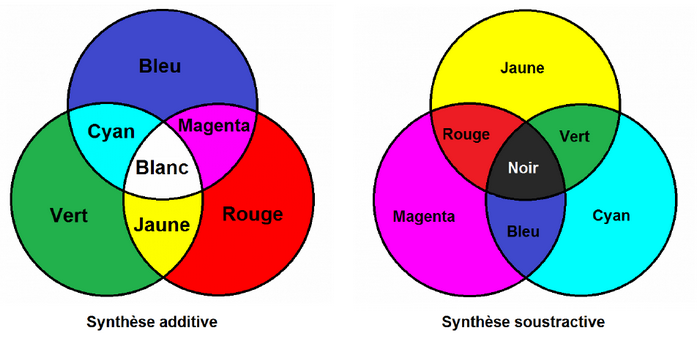
\includegraphics[scale = 0.7]{synthese_couleur.png}
	\caption{Gauche : synthèse additive. Droite : synthèse soustractive.}
	\end{center}
\end{figure}

Comment obtenir des couleurs ?\\

L'œil perçoit les objets grâce aux images qui se forment sur la rétine. Il perçoit les couleurs grâce
aux deux types de cellules photoréceptrices qu'il possède: les bâtonnets, très sensibles à l'intensité
lumineuse mais pas aux couleurs, et les cônes qui détectent les lumières colorées. Il existe trois types de cônes, chacun d'eux étant sensibles à une des trois couleurs primaires : rouge, vert ou
bleu.\\

En synthèse soustractive, la combinaison des couleurs cyan, magenta et jaune est suffisante pour recréer quasiment toutes les couleurs. On réalise une synthèse soustractive lorsqu'on supprime une partie du spectre d'une lumière pour obtenir une couleur différente. Quand on superpose plusieurs lumières colorées, le cerveau en perçoit une nouvelle : c'est la synthèse additive des couleurs. On obtient une infinité de couleurs en combinant les couleurs rouge, verte et bleue en proportions différentes.

\newpage
\subsection*{Acido-basicité de la phénolphtaléine}

\begin{figure}[h!]
	\begin{center}
  		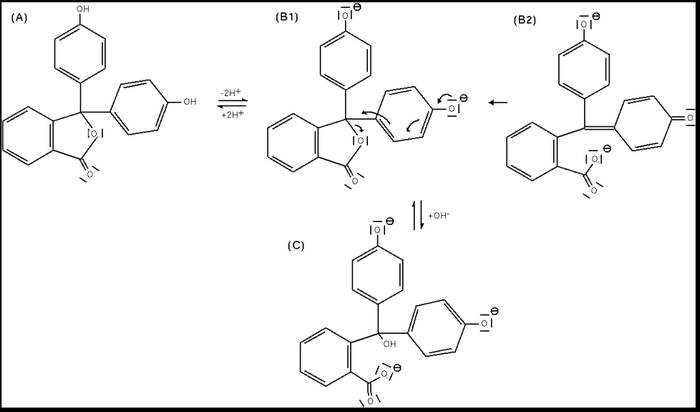
\includegraphics[scale = 0.7]{fifimeca.png}
	\caption{Gauche : synthèse additive. Droite : synthèse soustractive.}
	\end{center}
\end{figure}

En solution, la phénolphtaléine peut se présenter sous plusieurs formes en fonction de la quantité relative de base présente dans le milieu :
\begin{itemize}
	\item Pour des solutions acides : la phénolphtaléine est sous sa forme dite acide. La molécule 				possède un cycle de type lactone (A).
	\item Lors d'un ajout de base, le cycle lactone s'ouvre et évolue vers une structure 						triphénylcarbinol (non représentée) et cela amène la perte d'une molécule d'eau dans la 				structure et on forme une espèce ionique de couleur rouge pourpre (la longueur d'onde 					majoritairement absorbée se trouvant vers 550 nm). Cette espèce est décrite par deux formes 			mésomères (B1 et B2). La forme mésomère B2 laisse apparaître un système conjugué sur l'ensemble 		de la molécule. Ce système conjugué étendu est à l'origine de la coloration
	\item Pour un excès de base, la coloration pourpre disparait et le milieu redevient incolore 				traduisant la formation en solution du composé (C), ce composé ne possédant pas un système 				conjugué étendu.
\end{itemize}

\newpage
\subsection*{Les anthocyanes du jus de chou rouge}
\subsubsection{Matériel :}
\begin{itemize}
	\item Chou rouge
	\item Acide chlorhydrique
	\item Vinaigre d'alcool ou acide éthanoïque
	\item Jus de citron ou acide citrique
	\item Hydrogénocarbonate de sodium (bicarbonate de sodium)
	\item Solution aqueuse d'ammoniac
	\item Solution d'hydroxyde de sodium
	\item 9 tubes à essai, pipettes.
\end{itemize}

\subsubsection*{Protocole expérimental :}

\begin{itemize}
	\item \textbf{Préparation du jus de choux rouge}
	\begin{itemize}
		\item Mettre à chauffer 1 L d'eau (si possible distillée) dans une casserole;
		\item Couper la moitié d'un chou rouge en plusieurs morceaux et les mettre dans l'eau;
		\item Lorsque l'eau arrive à ébullition, arrêter de chauffer;
		\item Retirer les bouts de chou rouge, filtrer la solution à l'aide d'un filtre à café.
	\end{itemize}
	
	\item \textbf{Expériences avec les acides et les bases}
	\begin{itemize}
		\item Verser environ 5 mL de jus de chou rouge obtenu précédemment 
			dans 9 tubes à essai identiques.
		\item Diluer de moitié le contenu de chaque tube en ajoutant 5 mL d'eau. La couleur devrait 				être bleue. (Si ce n'est pas le cas, l'eau utilisée est peut-être légèrement acide ou 					basique ; ce n'est pas important pour la suite des expériences.)\\
		
		\item Tube 1 : ne rien y ajouter. Couleur de référence, "neutre", du chou rouge. Bleu.
		\item Tube 2 : une ou deux gouttes de jus de citron et mélanger. Rose-violet.
		\item Tube 3 : une ou deux gouttes d'acide éthanoïque (ou de vinaigre). Rose fuchsia.
		\item Tube 4 : une ou deux gouttes d'acide chlorhydrique. Rouge.
		\item Tube 5 : une dizaine de goutte d'acide chlorhydrique. Reste rouge et n'évolue plus.
		\item Tube 6 : pincée d'hydrogénocarbonate de sodium et agiter. Bleu-turquoise.
		\item Tube 7 : une goutte d'ammoniaque. Vert vif.
		\item Tube 8 : une goutte d'une solution d'hydroxyde de sodium. Jaune-vert.
		\item Tube 9 : plusieurs gouttes d'hydroxyde de sodium. Jaune vif et n'évolue plus.\\
		
		\item Tube 10 : ajouter une ou deux gouttes de vinaigre d'alcool. La couleur devient rose 						fuchsia. Ajouter quelques gouttes d'ammoniaque et constater que la couleur revient au 					bleu, puis devient d'un vert vif. Toujours dans ce tube, ajouter du vinaigre d'alcool 					et constater que la couleur peut repasser au bleu, puis au rose.
	\end{itemize}
\end{itemize}

\newpage
\subsection*{Mécanisme de la synthèse de l'indigo}

\end{document}